\section{Inference}
\label{sec:inference}

% \todo{PIC \textbf{Tomer A}}
\ourmodel inherits the inference-aware architecture of
\supermodel~\citep{nvidia2026nemotron3superopen}: LatentMoE~\citep{latentmoe_tr},
which buys more routed experts at fixed inference cost by trading away
hidden-dimension width; a hybrid Mamba-2 stack with sparse global Attention
anchors, which gives sub-quadratic sequence-length scaling during prefill
and a bounded KV-cache footprint during decode; and Multi-Token Prediction
for native speculative decoding (see \S\ref{sec:pretraining}). Below we first
characterize how these choices play out in practice across serving regimes ---
prefill- versus decode-heavy workloads and small- versus large-batch operation
--- and then turn to the considerations that come into focus when serving a
model of this size, considerations that did not bind at \supermodel{} or
\nanomodel{} scale.
Quantization recipes and the SSM-state cache treatment are covered in
\S\ref{sec:quantization}; headline throughput comparisons appear in
\S\ref{sec:intro}.

\subsection{Performance across serving regimes}
\label{sec:inference:regimes}
\ourmodel{}'s effective inference performance depends strongly on the
operating point: the prefill/decode balance of the workload and the batch
size at which it is served. We characterize both below.

\paragraph{Throughput across prefill- and decode-heavy workloads.}
\label{sec:inference:workloads}
Figure~\ref{fig:throughput_workloads} compares max-throughput serving on
GB200 NVL72 for two representative settings:
a decode-heavy 8K~input / 64K~output workload and a prefill-heavy
50K~input / 2K~output workload, both at NVFP4 precision with speculative
decoding disabled.
Prefill is compute-bound, so per-token cost tracks FLOPs, which are set by
the number of active parameters; \ourmodel{} pays roughly a $3.2\times$ FLOPs
penalty against Qwen-3.5-397B-17B (55B versus 17B active parameters), so the
MoE GEMMs are the dominant bottleneck and \ourmodel{} trails on the
prefill-heavy workload.
In large-batch decode, routing activates essentially all experts and per-step
cost is instead set by total weight I/O, where the gap shrinks to roughly
$1.39\times$ (550B versus 397B total parameters). With the MoE penalty that
much smaller, the token-mixing mechanism becomes the deciding factor, and
\ourmodel{}'s Mamba-2 state-space layers, whose per-step decode cost is
constant in sequence length, let it lead on the decode-heavy workload despite
trailing on prefill.

\begin{figure}[t]
    \centering
    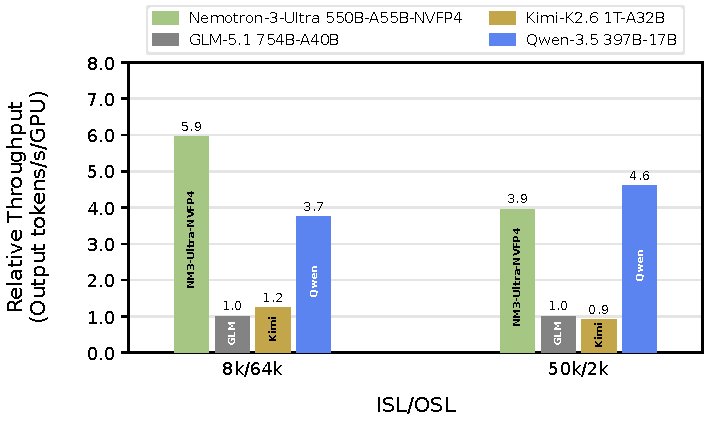
\includegraphics[width=0.7\linewidth]{figures/throughput_prefill_decode.pdf}
    \caption{Relative throughput on a decode-heavy (8K/64K) and a
    prefill-heavy (50K/2K) ISL/OSL setting, normalized to GLM-5.1 in both
    settings. The decode-heavy setting and measurement methodology match
    Figure~\ref{fig:intro}. \ourmodel{} leads on the decode-heavy setting
    ($1.6\times$ over Qwen-3.5) but trails Qwen-3.5 on the prefill-heavy
    setting, consistent with the active-parameter (prefill) versus
    total-weight-I/O (decode) analysis in the text.}
    \label{fig:throughput_workloads}
\end{figure}

\paragraph{Speculative decoding for hybrid models.}
Multi-Token Prediction (see \S\ref{sec:pretraining}) reduces main-model
forward passes at the cost of running the draft head and verifying
candidates. The operating point depends on batch size: at small batches
per-pass cost is dominated by weight reads, verification overhead is
cheap, and high draft length wins for latency; at large batches per-pass
cost is dominated by compute, verification overhead eats into
throughput, and lower draft lengths, or disabling MTP, often win.
We expose draft length as a deployment-time knob.
Figure~\ref{fig:mtp_dl_throughput} sweeps draft length on a
representative low-latency operating point: the NVFP4 checkpoint on a
single-user workload with ISL/OSL/BS = 10K/16K/1, on a single GB200
node at TP=4.

\begin{figure}[h]
    \centering
    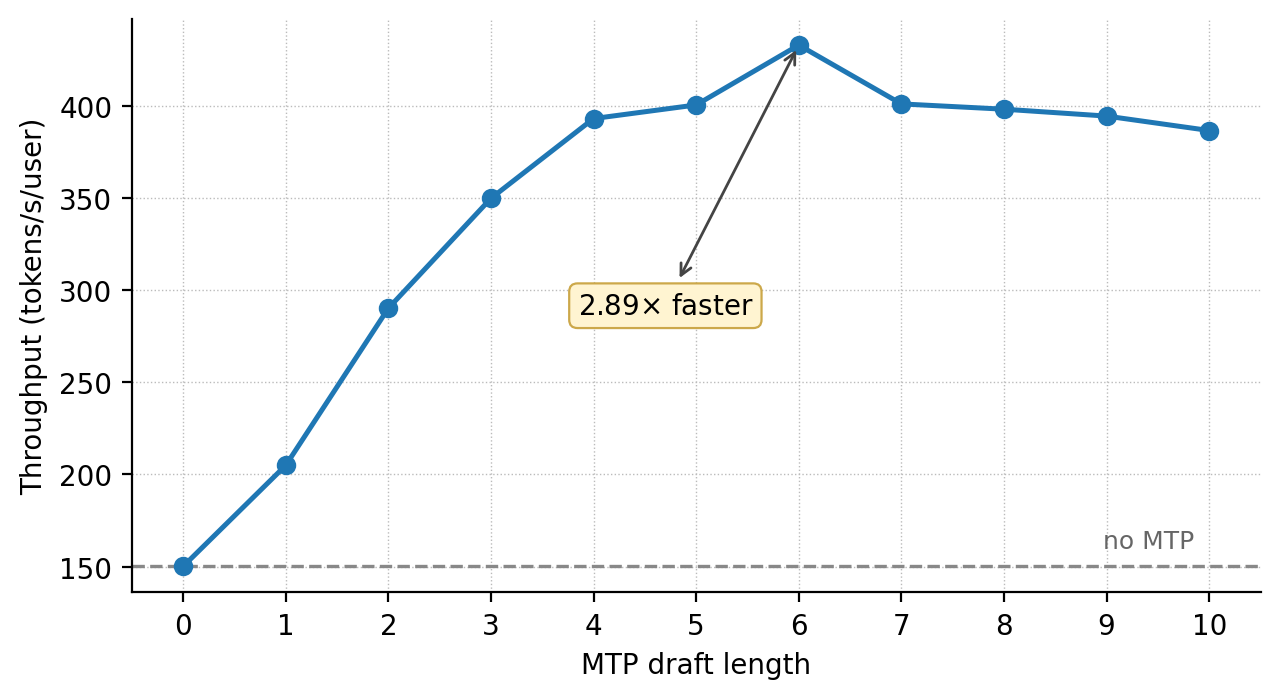
\includegraphics[width=0.55\linewidth]{figures/mtp_dl_throughput.png}
    \vspace{-0.5em}
    \caption{Decode throughput of the NVFP4 checkpoint as a function of
    MTP draft length on a single-user workload (ISL/OSL/BS = 10K/16K/1,
    single GB200 node, TP=4), using acceptance lengths measured on the
    SPEED-Bench benchmark~\citep{2026speedbench}. The dashed line is the no-MTP
    baseline; throughput peaks at DL=6, giving a $2.89\times$ speedup
    before gradually rolling off as verification overhead outweighs the
    marginal acceptance gain.}
    \label{fig:mtp_dl_throughput}
    \vspace{-0.5em}
\end{figure}
Hybrid Mamba models raise a second question: how to roll back state when
a draft token is rejected. For pure Attention this is a per-token KV
truncation; the Mamba SSM state, however, is a single fixed-size entry
per sequence that is overwritten every token, so no state corresponding
to an earlier token is directly available. We address this by
snapshotting the SSM state at every draft step. The same snapshotting
mechanism, run at a coarser cadence (every fixed number of tokens), also
gives us prefix caching across requests, otherwise unavailable for
Mamba, since prefix reuse in pure Attention is a free consequence of the
per-token KV cache.

\subsection{Inference at Ultra Scale}
\label{sec:inference:ultra-scale}

\paragraph{Parallelism choices and wide expert parallelism.}
\ourmodel{} is too large to fit on a single GPU and must be parallelized across
multiple ranks. The relevant axes are tensor parallelism (TP, which shards
the weight matrices of each linear layer across ranks), expert parallelism
(EP, which distributes full routed experts across ranks while Attention
and Mamba remain data-parallel), and combinations of the two, TP within
a group of ranks for Attention and Mamba, with routed experts EP-sharded
across and within those groups.
At small batch sizes inference is bound by weight-read memory bandwidth,
and wider TP wins: spreading weights across more ranks reduces per-step
HBM traffic by the TP factor, while the NVLink AllReduce of a single
hidden-state vector is negligible by comparison. At large batch sizes
communication of activation tensors becomes the bottleneck, and EP wins:
inter-rank traffic is confined to the all-to-all dispatch and combine that
bracket each routed-expert block, with no AllReduce on the critical path
of any GEMM, Attention, Mamba, and the routed experts all run
rank-local under EP.
For \ourmodel{}, this makes wide EP the practical choice for high-throughput
serving and wide TP the practical choice for low-latency serving; in some
low-latency settings we have also observed that combining TP and EP, 
along with DP for Attention and Mamba, outperforms either alone. Wide-EP serving in particular requires careful
load balancing across data-parallel ranks: because the routed-expert
all-to-all is synchronous, an under-loaded rank stalls the entire group,
so we route incoming requests to the least-loaded worker to keep per-rank
token counts close. Expert-level imbalance within each MoE layer can be
similarly addressed by replicating hot experts across EP ranks (EPLB). GB200 NVL72 is well-matched to all of these
configurations, most significantly for high-throughput: all 72 GPUs share
a single NVLink domain, so wide EP can span the full system without paying
for cross-domain interconnects in the all-to-all path. Wide TP benefits
from the same property for latency-bound serving, though only up to the
point at which per-rank weight reads shrink enough that AllReduce
becomes the new bottleneck.

\paragraph{Prefill-decode disaggregation for hybrid models.}
Prefill and decode stress the hardware very differently, as the workload
comparison above shows; serving both phases on a single replica therefore
forces a single parallelism configuration and scheduling policy across two
workloads with very different requirements.
Prefill-decode disaggregation, which runs the two phases on separate
workers with their own parallelism and scheduling, is the established
response, and we adopt it for \ourmodel{}. Disaggregation requires transferring
the KV cache from prefill to decode workers on every request; for hybrid
Mamba-Attention models extra care is needed to ensure both the KV cache
and the Mamba SSM state are transferred correctly, and that consumers of
cache-state events can tell the two apart. We landed the necessary
upstream changes, including the semantic KV-event metadata path that
identifies hybrid cache groups and the NIXL side-channel host-resolution
fix needed for multi-node Ray, and disaggregation for hybrid
Mamba-Attention models now works out-of-the-box in
vLLM~\citep{kwon2023efficientmemorymanagementlarge}. End-to-end we
currently measure up to roughly 10\% throughput improvement from
disaggregation on \ourmodel{} on prefill-heavy workloads, and expect
further gains as the software stack matures.

\paragraph{All-to-all backend.}
Under expert parallelism, the routed-expert all-to-all is the dominant
inter-rank communication during MoE serving. It accounts for roughly
15\% to 20\% of total runtime on prefill-heavy workloads
(50K input / 2K output tokens). The default vLLM scheme implements this all-to-all as an AllGather of
activations followed by a ReduceScatter of expert outputs, simple,
dependency-free, and topology-agnostic, but intrinsically wasteful:
AllGather replicates every token on every rank, when each rank only
needs the subset routed to its experts. We
evaluated several true all-to-all backends and adopted FlashInfer's
NVLinkOneSided implementation~\citep{nvidia2026nvlinkonesided} as the
best end-to-end choice for \ourmodel{} serving on GB200 NVL72. End-to-end we measure roughly 5\% throughput
improvement from this backend over the default vLLM scheme; performance
analysis indicates the all-to-all kernel itself still has room for
further optimization. A more fundamental alternative is to avoid the
all-to-all altogether: DWDP~\citep{nvidia2026dwdp} keeps execution
data-parallel and instead pulls each layer's expert weights to every rank,
prefetched behind the preceding compute so the transfer is hidden.

\paragraph{Prefill and MoE chunking.}
On prefill-heavy workloads (e.g.\ 50K input / 2K output), the natural
scheduling choice is to chunk prefill at the request level so chunks
can be interleaved with decode forward passes. Small chunks at
moderate-to-high batch sizes leave essentially no pure-decode passes,
hurting user interactivity (TPOT), and at large batch sizes the number
of prefill passes per request can exceed the number of decode passes.
Growing the chunk size resolves this, but exposes a second issue under
wide expert parallelism: while Attention and Mamba are DP-sharded and
each rank processes only $\text{concurrency} / \text{DP}$ requests,
the routed-expert kernels process the union of tokens from all
data-parallel ranks. Large prefill chunks therefore drive the routed-expert kernels into a
regime where kernel-level resource limits become binding. The fix is
MoE-side chunking, splitting the token batch within the MoE kernel
itself, so chunk size can grow without hitting these limits. We
landed this fix upstream in vLLM.

\paragraph{GEMM dimensions and weight padding.}
Several combinations of tensor parallelism factor, quantization format,
and target hardware land the per-rank GEMM dimensions at sizes that
violate kernel alignment requirements. In every such case the route we
have taken is to pad the affected weight matrices at load time so the
kernel sees an acceptable shape, with runtime infrastructure adjusted
to ignore the padded positions. Examples include MoE NVFP4 kernels
whose hidden- or intermediate-dimension alignment requirements exceed
what naturally falls out of the architecture, and Marlin NVFP4 linear
and MoE kernels on Hopper that impose tile- and thread-level alignment
constraints on their inputs. A natural improvement for future model
generations is to choose the model's inner dimensions such that all
expected (TP, quantization, hardware) tuples produce kernel-friendly
shapes without requiring load-time padding.
